The last section was all about running multiple threads on the same machine without any interaction between these threads. If you can split the work your program does between threads in a way that makes such implementation possible, by all means, do it. You cannot beat the performance of such an embarrassingly parallel program.

More often than not, threads must interact with each other because they are contributing work to a common result. Such interactions happen by means of threads communicating with each other through the one resource they share, the memory. We must now understand the performance implications of this.

Let us start with a trivial example. Say we want to compute a sum of many values. We have many numbers to add, but, in the end, only one result. We have so many numbers to add that we want to split the work of adding them between several threads. But there is only one result value, so the threads have to interact with each other as they add to this value.

\hspace*{\fill} \\ %插入空行
\noindent
\textbf{02\_sharing\_incr.C}
\begin{lstlisting}[style=styleCXX]
unsigned long x {0};
void BM_incr(benchmark::State& state) {
	for (auto _ : state) {
		benchmark::DoNotOptimize(++x);
	}
}
BENCHMARK(BM_incr)->Threads(2);
\end{lstlisting}

For simplicity, we always increment the result by 1 (the cost of adding integers does not depend on the values, and we don't want to benchmark the generation of different values, just the addition itself). Since the benchmark function is called by each thread, any variable declared inside this function exists independently on the stack of each thread; these variables are not shared at all. To have a common result that both threads contribute to, the variable must be declared outside of the benchmark function, at the file scope (bad idea in general, but necessary and acceptable in the very limited context of the microbenchmark).

Of course, this program has a much bigger problem than the global variable: the program is simply wrong, and its results are undefined. The problem is that we have two threads incrementing the same value. Incrementing a value is a 3-step process: the program reads the value from memory, increments it in the register, and writes the new value back into memory. It is entirely possible for both threads to read the same value (0) at the same time, increment it separately on each processor (1), and write it back. The thread that writes second simply overwrites the result of the first thread, and, after two increments, the result is 1 instead of 2. Such competition of two threads for writing into the same memory location is called a data race. 

Now that you understand why such unguarded concurrent accesses are a problem, you may as well forget it; instead, follow this general rule: any program has undefined results if it accesses the same memory location from multiple threads without synchronization and at least one of these accesses is a write. This is very important: it is not necessary for you to figure out exactly what sequence of operations must happen for the result to be incorrect. In fact, there is nothing to be gained in this line of reasoning at all. Any time you have two or more threads accessing the same memory location, you have a data race unless you can guarantee one of two things: either all accesses are read-only, or all accesses use the correct memory synchronization (which we are yet to learn about).

Our problem of computing the sum requires that we write the answer into the result variable, so the access is definitely not read-only. The synchronization of memory accesses is, in general, provided by a mutex: every access to a variable shared between threads must be guarded by a mutex (it must, of course, be the same mutex for all threads).

\hspace*{\fill} \\ %插入空行
\noindent
\textbf{03\_mutex\_incr.C}
\begin{lstlisting}[style=styleCXX]
unsigned long x {0};
std::mutex m;

{ // Concurrent access happens here
	std::lock_guard<std::mutex> guard(m);
	++x;
}
\end{lstlisting}

The lock guard locks the mutex in its constructor and unlocks it in the destructor. Only one thread at a time can have the lock and, thus, increment the shared result variable. The other threads are blocked on the lock until the first thread releases it. Note that all accesses must be locked, both reads and writes, as long as at least one thread is modifying the variable.

Locks are the simplest way to ensure the correctness of a multi-threaded program, but they are not the easiest thing to study in terms of performance. They are fairly complex entities and often involve a system call. We will start with a synchronization option that is, in this particular case, easier to analyze: the atomic variable.

C++ gives us an option to declare a variable to be atomic. It means that all supported operations on this variable are performed as single, non-interruptible, atomic transactions: any other thread observing this variable will see its state either before the atomic operation or after it, but never in the middle of the operation. For example, all integer atomic variables in C++ support atomic increment operations: if one thread is executing the operation, no other thread can access this variable until the first operation is complete. These operations require certain hardware support: for example, the atomic increment is a special hardware instruction that reads the old value, increments it, and writes the new value all as a single hardware operation.

For our example, an atomic increment is all we need. It must be stressed that, whatever synchronization mechanism we decided to use, all threads must use the same mechanism for concurrent accesses to a particular memory location. If we use atomic operations on one thread, it guarantees no data races as long as all threads use atomic operations. If another thread uses a mutex or non-atomic access, all guarantees are void, and the result is undefined again.

Let us rewrite our benchmark to use C++ atomic operations:

\hspace*{\fill} \\ %插入空行
\noindent
\textbf{02\_sharing\_incr.C}
\begin{lstlisting}[style=styleCXX]
std::atomic<unsigned long> x(0);
void BM_shared(benchmark::State& state) {
	for (auto _ : state) {
		benchmark::DoNotOptimize(++x);
	}
}
\end{lstlisting}

The program is now correct: there are no data races here. It is not necessarily accurate since a single increment is a very short time interval to measure; we really should unroll the loop manually or with a macro and do several increments per loop iteration (we have done that in the last chapter, so you can see the macro there). Let us see how well it performs. If there were no interaction between the threads, two threads would compute the sum in half the time it takes one thread to do it:

\hspace*{\fill} \\ %插入空行
\begin{center}
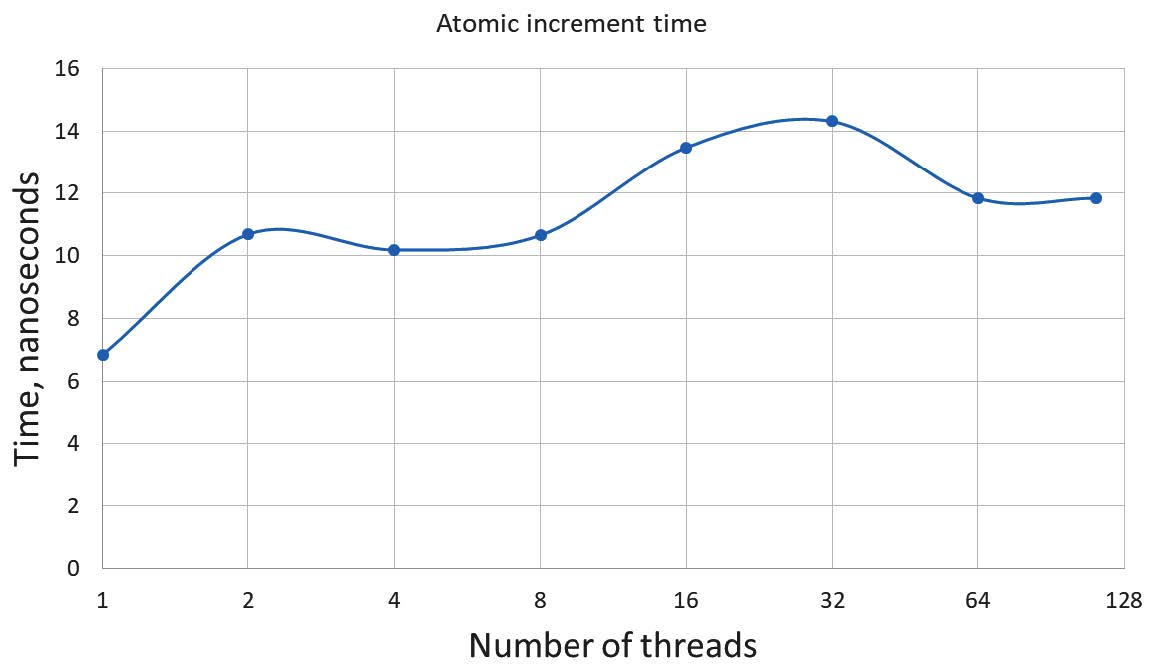
\includegraphics[width=0.9\textwidth]{content/1/chapter5/images/4.jpg}\\
Figure 5.4 – Atomic increment time in a multi-threaded program
\end{center}

We have normalized the results to show the average time of a single increment, that is, the time to compute the sum divided by the total number of additions. The performance of this program is very disappointing: not only is there no improvement, but, in fact, it takes longer to compute the sum on two threads than on one.

The results are even worse if we use the more conventional mutex:

\hspace*{\fill} \\ %插入空行
\begin{center}
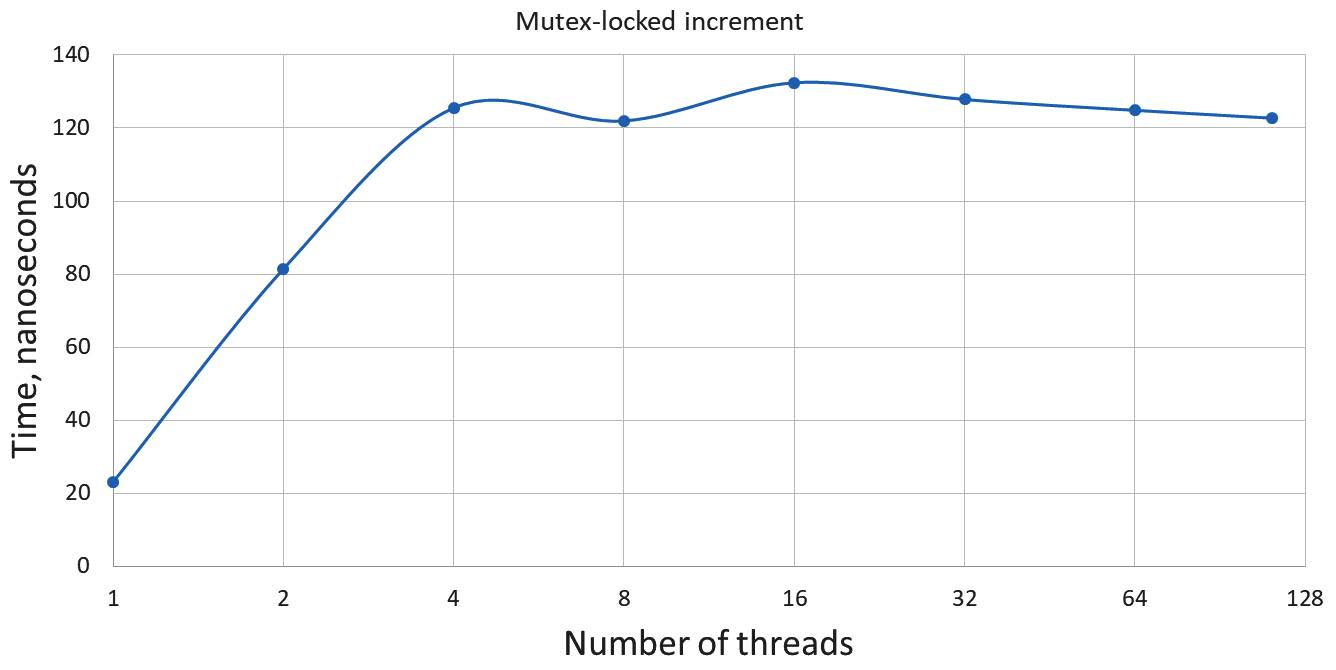
\includegraphics[width=0.9\textwidth]{content/1/chapter5/images/5.jpg}\\
Figure 5.5 – Increment time in a multi-threaded program with a mutex
\end{center}

First of all, as we expected, locking the mutex is a fairly expensive operation even on one thread: 23 nanoseconds for a mutex-guarded increment versus 7 nanoseconds for the atomic increment. The performance degrades much faster as the number of threads increases.

There is a very important lesson to be learned from these experiments. The portion of the program that accesses the shared data will never scale. The best performance you can have for accessing the shared data is single-threaded performance. As soon as you have two or more threads accessing the same data at the same time, the performance can only get worse. Of course, if two threads are accessing the same data at different times, they don't really interact with each other, so you get the single-threaded performance both times. The performance advantage of a multi-threaded program comes from the computations that the threads do independently, without synchronization. By definition, such computations are done on data that is not shared (if you want your program to be correct, anyway). But why are concurrent accesses to the shared data so expensive? In the next section, we will learn the reason. We will also learn a very important lesson on carefully interpreting measurements.








